Nous souhaitons non seulement v\'erifier if $G_M$ est un line-graphe mais aussi trouver le graphe racine de $G_M$, un DAG modelis\'e par un r\'eseau \'electrique sans ambiguit\'e.
\newline 
\begin{definition}
	Le graphe $G_M$ est un graphe de corr\'elation ssi il est le line graphe d'un DAG.
\end{definition}
D'apr\`es le theor\`eme \ref{caracteristiquesLinegraphes}, L'ensemble des cliques $\cal C$ est dit une {\bf couverture de corr\'elation} de $G_M$.

\begin{definition}
Une ambigu\"{i}t\'e est un graphe isomorphe \`a l'un des graphes de la figure \ref{configurationAmbiguite}. Le sommet $X$ est appel\'e le {\bf point d'ambiguit\'e}.
\end{definition}

\begin{figure}[htb!]\vspace{-0.5em}
	\centering
	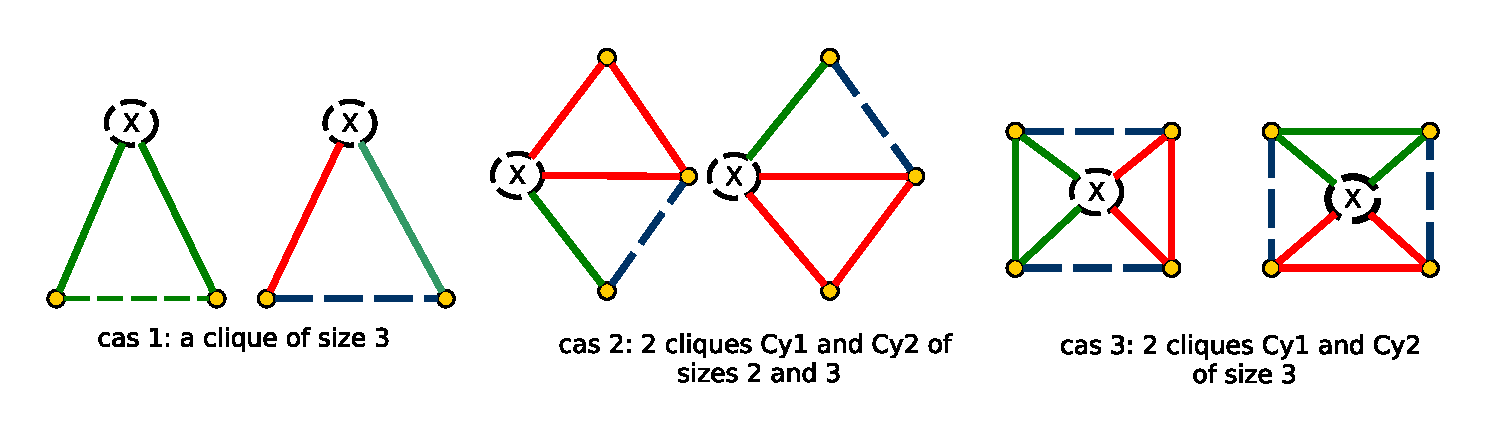
\includegraphics[scale=0.70]{configurationAmbiguite.eps}\vspace{-0.5em}
	\caption{ Configurations possibles d'une ambiguit\'e au sommet X }\vspace{-0.5em}
	\label{configurationAmbiguite}
\end{figure}

\begin{lemma}
	Si un graphe de corr\'elation $G_M$ admet deux couvertures de corr\'elation, alors il existe au moins un sommet $u$ de $G_C$ tel que $G_{C}[\{u\} \cup \Gamma_{G_C}(u)]$ est une ambiguit\'e dont $u$ est le point.
\end{lemma}
	
\begin{proof} 
	Consid\'erons deux line-couvertures $C$ et $C'$ de $G_C$. 
	Il existe au moins un sommet $v \in G_C[V]$ qui n'est pas couvert par la (ou les) m\^eme(s) clique(s) dans $C$ et $C'$.
	Soient deux cliques $c_1$ et $c_2$ (potentiellement vide) partitionant $\{v\} \cup \Gamma_{G_C}(v)$ dans $\cal C$.
	Consid\'erons deux autres cliques $c_3$ et $c_4$ diff\'erentes de $c_1$ et $c_2$ partitionant \'egalement $\{v\} \cup \Gamma_{G_C}(v)$ dans $\cal C$. \newline
	Notons $c_{i,j}$ l'intersection de $c_{i}$ et $c_j$ pour tout $i \in \{1,2\}$ et $j \in \{3,4\}$. 
	Chaque sommet $w \in c_{i,j}$ est couvert par au plus deux cliques de $G$ dans $\cal C$, dont la clique $c_i$.
	Puisque $c_j$ est une clique alors ce sommet $w$ est voisin de tous les sommets de  $c_{i',j}$, pour $i' \ne i$.
	Les ar\^etes entre ces sommets sont dans $c'_i$, donc chaque ar\^ete $[w,z]$ pour tout sommet  $z \in c_{i',j}$ forme une clique correspondant dans le r\'eseau de flots.
	Ainsi, le cardinal de chaque ensemble  $c_{i,j}$ est \'egal \`a $1$.\newline
	Appelons $v_{i,j}$ le seul sommet pr\'esent dans $c_{i,j}$. 
	Il est possible d'avoir $v_{1,3} = v_{1,4}$ ou $v_{2,3} = v_{2,4}$.
	Si les deux \'egalit\'es sont v\'erifi\'ees, le sommet $v$ est alors couvert non pas par deux cliques mais par une seule de cardinalit\'e $3$.
	Ainsi, les seuls cas possibles sont alors r\'esum\'es par la figure  \ref{graphe2Couverture}.
	Le sommet $v$ est bien le point d'une ambigu\"{i}t\'e isomorphe \`a $G_C[\{u\} \cup \Gamma_{G_C}(u)]$.
\end{proof}

Nous d\'eduisons le corollaire suivant :
\begin{corollary}
Si un graphe de corr\'elation admet deux couvertures de corr\'elation, alors il est isomorphe \`a l'un des graphes de la figure  \ref{graphe2Couverture}.
\end{corollary}

\begin{figure}[htb!] \vspace{-0.5em}
\centering
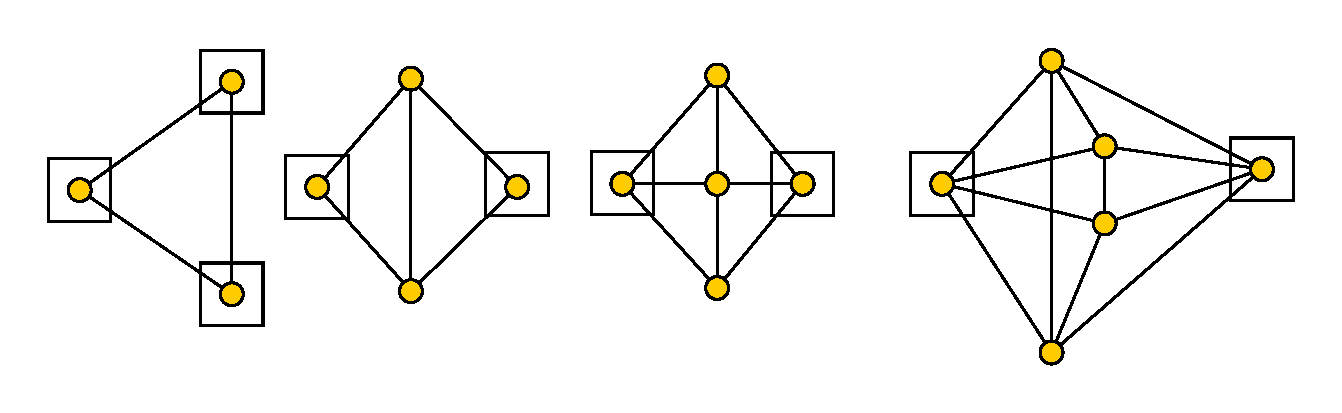
\includegraphics[scale=0.75]{graphe2Couverture.eps}
\caption{ Graphes possibles avec deux couvertures avec les points d'ambigu\"{i}t\'es }
\label{graphe2Couverture} 
\end{figure}
En Effet, si $G_M[\{u\} \cup \Gamma_{G_M}(u)]$ est une ambigu\"{i}t\'e, chaque ar\^ete, qui n'est pas li\'ee au point d'ambigu\"{i}t\'e, doit \^etre une ar\^ete d'une et une seule autre ambigu\"{i}t\'e de $G_M$. Et chaque sommet d'une ambigu\"{i}t\'e, qui n'est pas un point d'ambigu\"{i}t\'e, doit appartenir \`a une et une seule autre ambigu\"{i}t\'e de $G_M$ dont il n'est pas non  plus le point d'ambigu\"{i}t\'e.
De plus, chaque ar\^ete, n'\'etant pas couvert par les deux configurations de cliques possibles dans une ambigu\"{i}t\'e (les ar\^etes en pointill\'ees dans la figure \ref{graphe2Couverture}), doivent \^etre dans la m\^eme situation dans une autre ambigu\"{i}t\'e \`a laquelle elles appartiennent.
Ces contraintes font que si un graphe contient une ambigu\"{i}t\'e induite, alors il ne peut \^etre que dans un cas de la figure  \ref{graphe2Couverture}.

\begin{definition}
Soit $G$ un graphe et $u$ un sommet de $G$. Une partition de $\Gamma_G(v)$ en deux cliques $C_{u1}, C_{u2}$ est {\bf coh\'erente } ssi chaque sommet $v$ de $C_{u1}$ (resp $C_{u2}$) a au plus un voisin dans $C_{u2}$  (resp $C_{u1}$).
\end{definition}
Le r\'esultat suivant est un corollaire direct de la preuve du lemme \ref{lemmaCoherente}
\begin{lemma}
\label{lemmaCoherente}
Soit $G_M$ un line graphe, $u$ un sommet de $G_M$ et une partition coh\'erente de ${u} \cup \Gamma_{G_M}(v)$ en deux cliques  $C_{u1}, C_{u2}$. 
Si l'une de ces deux cliques est de cardinal sup\'erieur ou \'egal \`a $4$, alors cette partition coh\'erente est unique.
\end{lemma}

\'Etant donn\'e une partition coh\'erente $C_{u1}, C_{u2}$ pour un sommet $u$ de $G_M$, la fiabilit\'e de cette coh\'erence est
$$F(C_{u1}, C_{u2}) = \min\limits_{[x,y] \in E(C_{u1}) \cup E(C_{u2})}  \mu_{C}([x,y])$$


Une {\bf line-couverture} d'un graphe non orient\'e connexe $G_C$ est un ensemble de cliques maximales de $G_M$ telles que chaque sommet de $G_C$ appartient \`a une ou deux de ces cliques et que chaque ar\^ete de $G_C$ soit couverte par exactement une de ces cliques.
s'il existe une line-couverture de $G_M$ alors nous supposons que $G_M$ est le v\'eritable  line-graphe du DAG $G$ du r\'eseau \'electrique.
Dans le cas $G_M$ n'est pas un line-graphe alors nous d\'eterminons le line-graphe $G'$ avec le m\^eme ensemble de sommets que $G_M$ minimisant la distance avec $G_M$ d\'efinie dans la partie suivante.
